\documentclass[a4paper, 12pt]{article}%тип документа

%отступы
\usepackage[left=2cm,right=2cm,top=2cm,bottom=3cm,bindingoffset=0cm]{geometry}

%Русский язык
\usepackage[T2A]{fontenc} %кодировка
\usepackage[utf8]{inputenc} %кодировка исходного кода
\usepackage[english,russian]{babel} %локализация и переносы

%Вставка картинок
\usepackage{graphicx}
\graphicspath{{pictures/}}
\DeclareGraphicsExtensions{.pdf,.png,.jpg}

%Графики
\usepackage{multirow}
\usepackage{pgfplots}
\pgfplotsset{compat=1.9}

%Римские цифры
\newcommand{\RNumb}[1]{\uppercase\expandafter{\romannumeral #1\relax}}

%Математика
\usepackage{amsmath, amsfonts, amssymb, amsthm, mathtools}

%Заголовок
\author{Богданов Александр \\
	Б05-003}
\title{\textbf{Работа 5.(2.2 - 2.3) \\ 
		Излучение атома водорода и молекулы йода}}

\begin{document}

\maketitle

\textbf{Цель работы:} исследовать спектральные закономерности в оптическом спектре водорода; вычислить постоянную Ридберга; исследовать спектр поглощения паров йода в видимой области; вычислить энергию колебательного кванта молекулы йода и энергию ее диссоциации в основном и возбужденном состояниях.

\textbf{В работе используются:} стеклянно-призменный монохроматор-спектрометр УМ-2; ртутная лампа ПРК-4; неоновая лампа; водородная лампа.\\

\textbf{Теоретические положения:}\\\par

\textbf{Спектр атома водорода}

	Длины волн спектральных линий водородоподобного атома описываются формулой:
	
\[\frac{1}{\lambda_{mn}} = R Z^2 \left( \dfrac{1}{n^2} - \dfrac{1}{m^2}\right),\]

где $R$ -- константа (постоянной Ридберга),  $Z$ -- порядковый номер атома,  а $m$ и $n$ -- целые числа.

	\begin{figure}[h!]
		\centering
		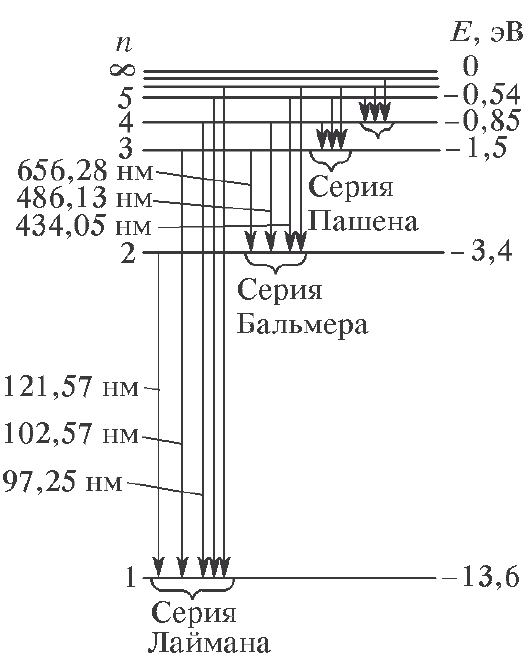
\includegraphics[scale=0.4]{Схема_1.PNG}
		\caption{Уровни энергии атома водорода и образование спектральных серий}
	\end{figure}

Если считать ядро неподвижным,  то возможные энергетические состояния водородоподобного атома определяются выражением:

\[E_n = - \frac{2 \pi^2 m_e e^4 Z^2}{h^2} \frac{1}{n^2}.\]

	Из схемы видно,  что линии в спектре водорода можно расположить по сериям; для всех линий серии значение $n$ остается постоянным,  а $m$ может принимать любые значения от $n+1$ до $\infty$.

В данной работе изучается серия Бальмера,  линии которой лежат в видимой области.  Для серии Бальмера $n = 2$.  Величина $m$ для первых четырех линий этой серии принимает значение 3,  4,  5,  6.  Эти линии обозначаются символами $H_{\alpha},  H_{\beta},  H_{\gamma},  H_{\delta}$.\\

\textbf{Спектр молекулы йода}

В первом приближении энергия молекулы может быть представлена в виде:

\[E = E_{\text{эл}} + E_{\text{колеб}} + E_{\text{вращ}},\]

	где $E_{\text{эл}},  E_{\text{колеб}}$ и $E_{\text{вращ}}$ -- электронная, колебательная и вращательная энергии молекулы соответственно.

	Оптические переходы (переходы, связанные с излучением фотонов в видимом диапазоне длин волн) соответствуют переходам между различными электронными состояниями молекулы.  При этом обычно происходят также изменения ее вращательного и колебательного состояний,  однако наблюдение первых оптическими спектрометрами невозможно в силу малости их энергии.

	\begin{figure}[h!]
		\centering
		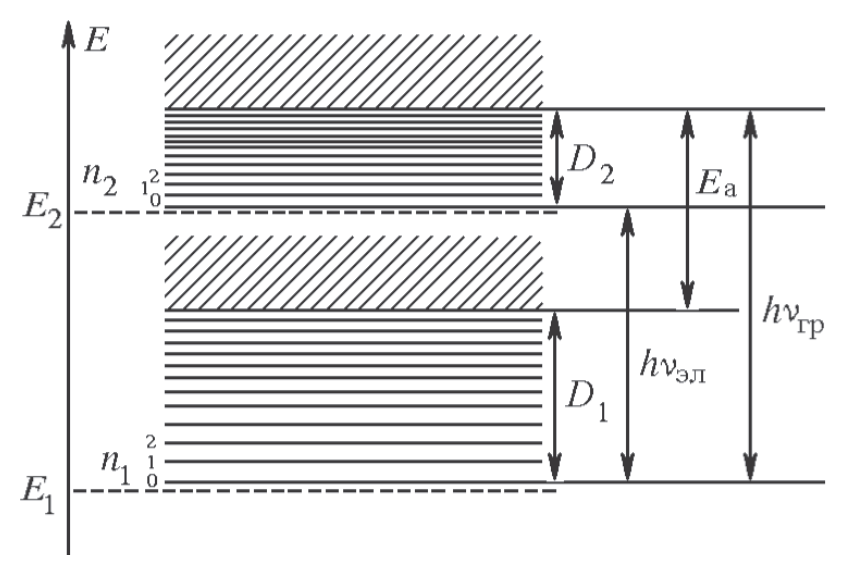
\includegraphics[scale=0.4]{Схема_2.PNG}
		 \caption{Электронные и электронно-колебательные энергетические уровни двухатомной молекулы}
	\end{figure}

	На схеме изображены энергетические уровни молекулы без учета вращательной структуры.  Штриховыми линиями показаны чисто электронные уровни $E_1$ и $E_2$,  а сплошными --  колебательные подуровни этих состояний.  Следует подчеркнуть,  что минимальное значение колебательной энергии при $n = 0$ отлично от нуля и равно $h \nu / 2$.

	Наименьшая энергия,  которую нужно сообщить молекуле в нижайшем колебательном состоянии,  чтобы она диссоциировала,  называется энергией диссоциации.  На схеме $E_{\text{а}}$ -- энергия возбуждения атома,  возникающая при переходе молекулы из состояния 1 в область непрерывного спектра,  соответствующего состоянию 2.  Энергия чисто электронного перехода $E_2 - E_1 = h\nu_{\text{эл}}$.  Границу схождения спектра,  т.е.  энергию возбуждения,  при которой происходит переход молекулы в область непрерывного спектра,  обозначим через $h \nu_{\text{гр}}$. 

	\begin{figure}[h!]
		\centering
		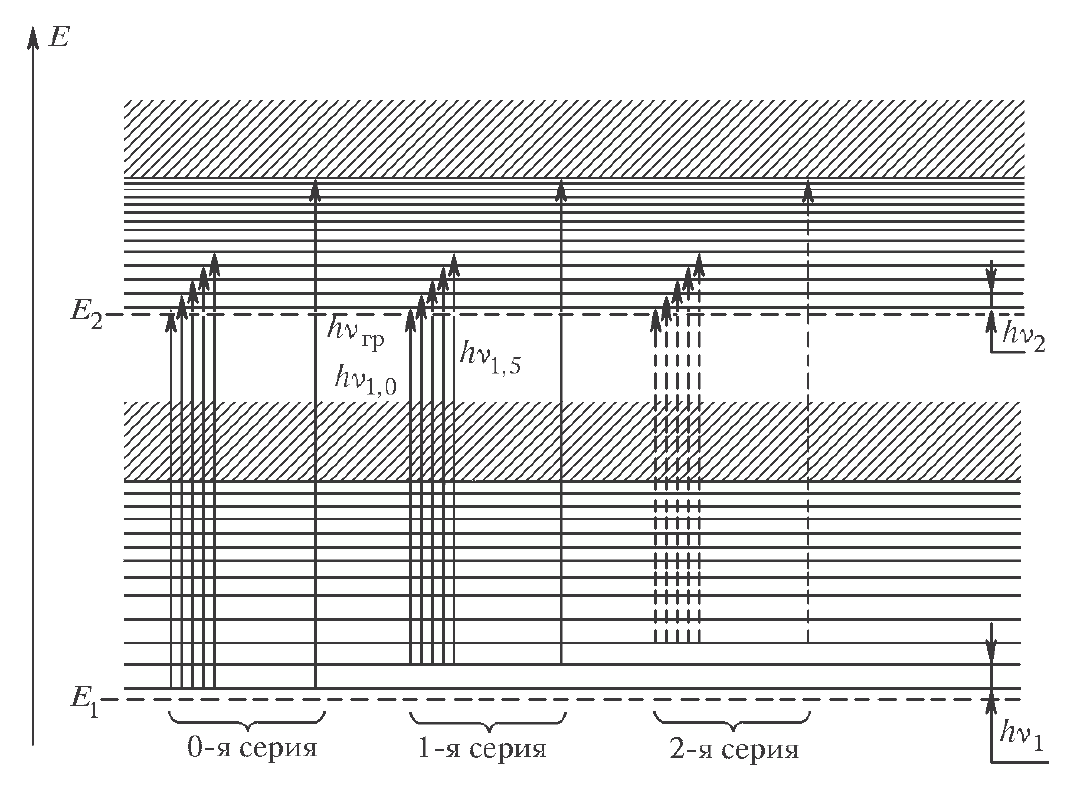
\includegraphics[scale=0.35]{Схема_3.PNG}
		\caption{Структура электронно-колебательного спектра поглощения молекулы йода в видимой области}
	\end{figure}

	На схеме показана структура электронно-колебательного спектра поглощения молекул йода,  который исследуется в данной работе.  Серии,  указанные на схеме,  называются сериями Деландра.  Энергетические расстояния между линиями в начале серии приблизительно равны:

\[h \nu_{0, n_2} - h \nu_{0, (n_2 - 1)} \approx h \nu_2,\]

т.е.  они равны колебательному кванту в возбужденном электронном состоянии.

	\begin{figure}[h!]
		\centering
		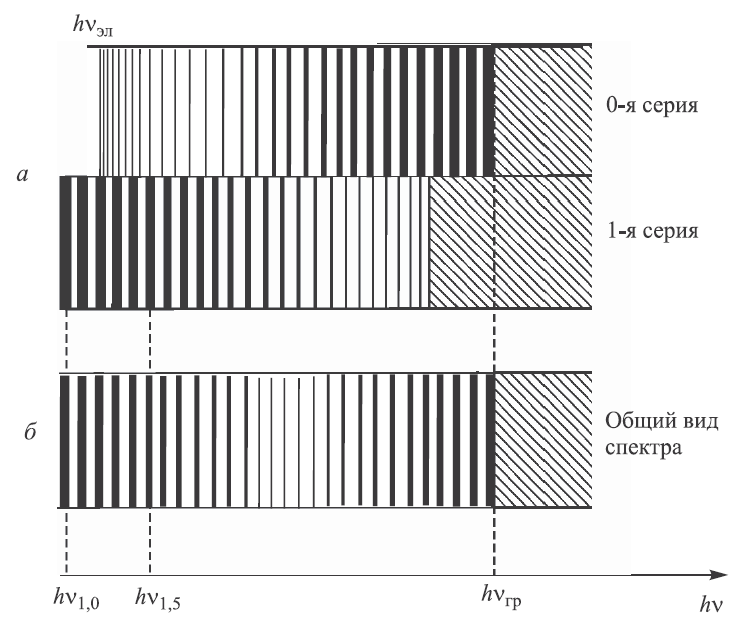
\includegraphics[scale=0.45]{Схема_4.PNG}
		\caption{Спектр поглощения паров йода}
	\end{figure}

	Общий вид спектра показан на схеме.  Из рассмотренного ясно,  что спектр поглощения паров йода в видимой области при температуре $T \approx 300 \text{ К}$ практически состоит из двух серий Деландра (1-й и 0-й),  накладывающихся друг на друга. 
	
\textbf{Экспериментальная установка:}\\\par

	\begin{figure}[h!]
		\centering
		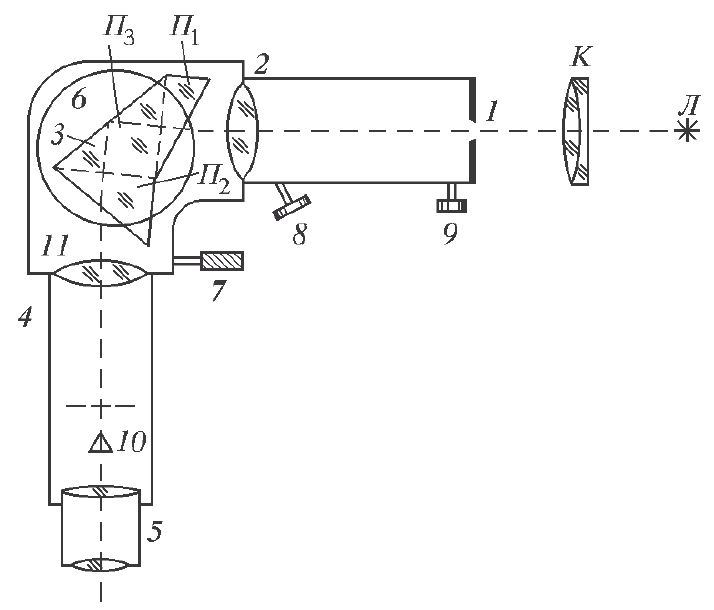
\includegraphics[scale=0.45]{Установка_1.PNG}
		\caption{Устройство монохроматора УМ-2}
	\end{figure}

	Для измерения длин волн спектральных линий в работе используется стеклянно-призменный монохроматор-спектрометр УМ-2.  Основные элементы монохроматора представлены на схеме.

	Спектрометр УМ-2 нуждается в предварительной градуировке.  Для градуировки в коротковолновой части спектра удобно применять ртутную лампу ПРК-4,  а в длинноволновой и средней части спектра -- неоновую лампу.  Таблицы спектральных линий ртути и неона с визуальной оценкой их относительной интенсивности приведены на установке:

	\begin{figure}[h!]
		\centering
		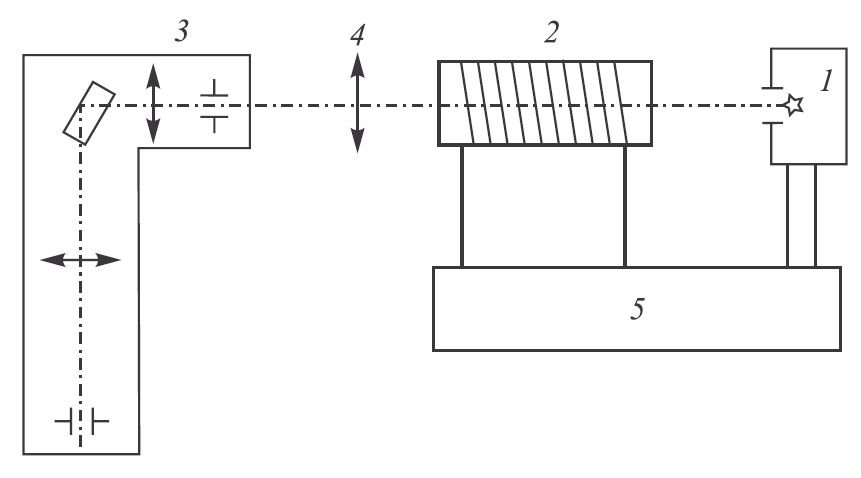
\includegraphics[scale=0.45]{Установка_2.PNG}
		\caption{Схема экспериментальной установки}
	\end{figure}

	В нашей работе спектр поглощения паров йода наблюдается визуально на фоне сплошного спектра лампы накаливания 1,  питаемой от блока питания 2.  Кювета 3 с кристаллами йода подогревается нихромовой спиралью, подключенной вместе с лампой накаливания к блоку питания. Линза 4 используется как конденсор.\\

\textbf{Ход работы:}\\\par

\begin{enumerate}

\item Настроим установку.

\item Произведём градуировку монохроматора.  Для этого проведём измерения линий спектра неона и ртути,  сняв зависимость длины волны наблюдаемого света $\lambda$ от параметра $\theta$ барабана монохроматора:

	\begin{figure}[h!]
		\centering
		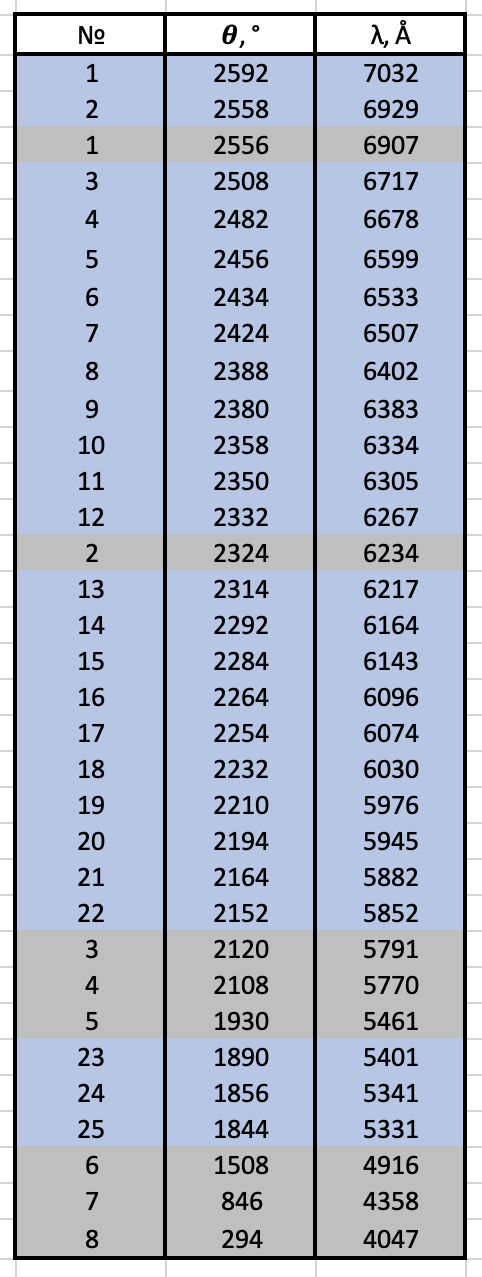
\includegraphics[scale=0.8]{Таблица_1.PNG}
		\caption{Голубой -- неон,  серый -- йод}
	\end{figure}

\newpage
	
	\begin{figure}[h!]
		\centering
		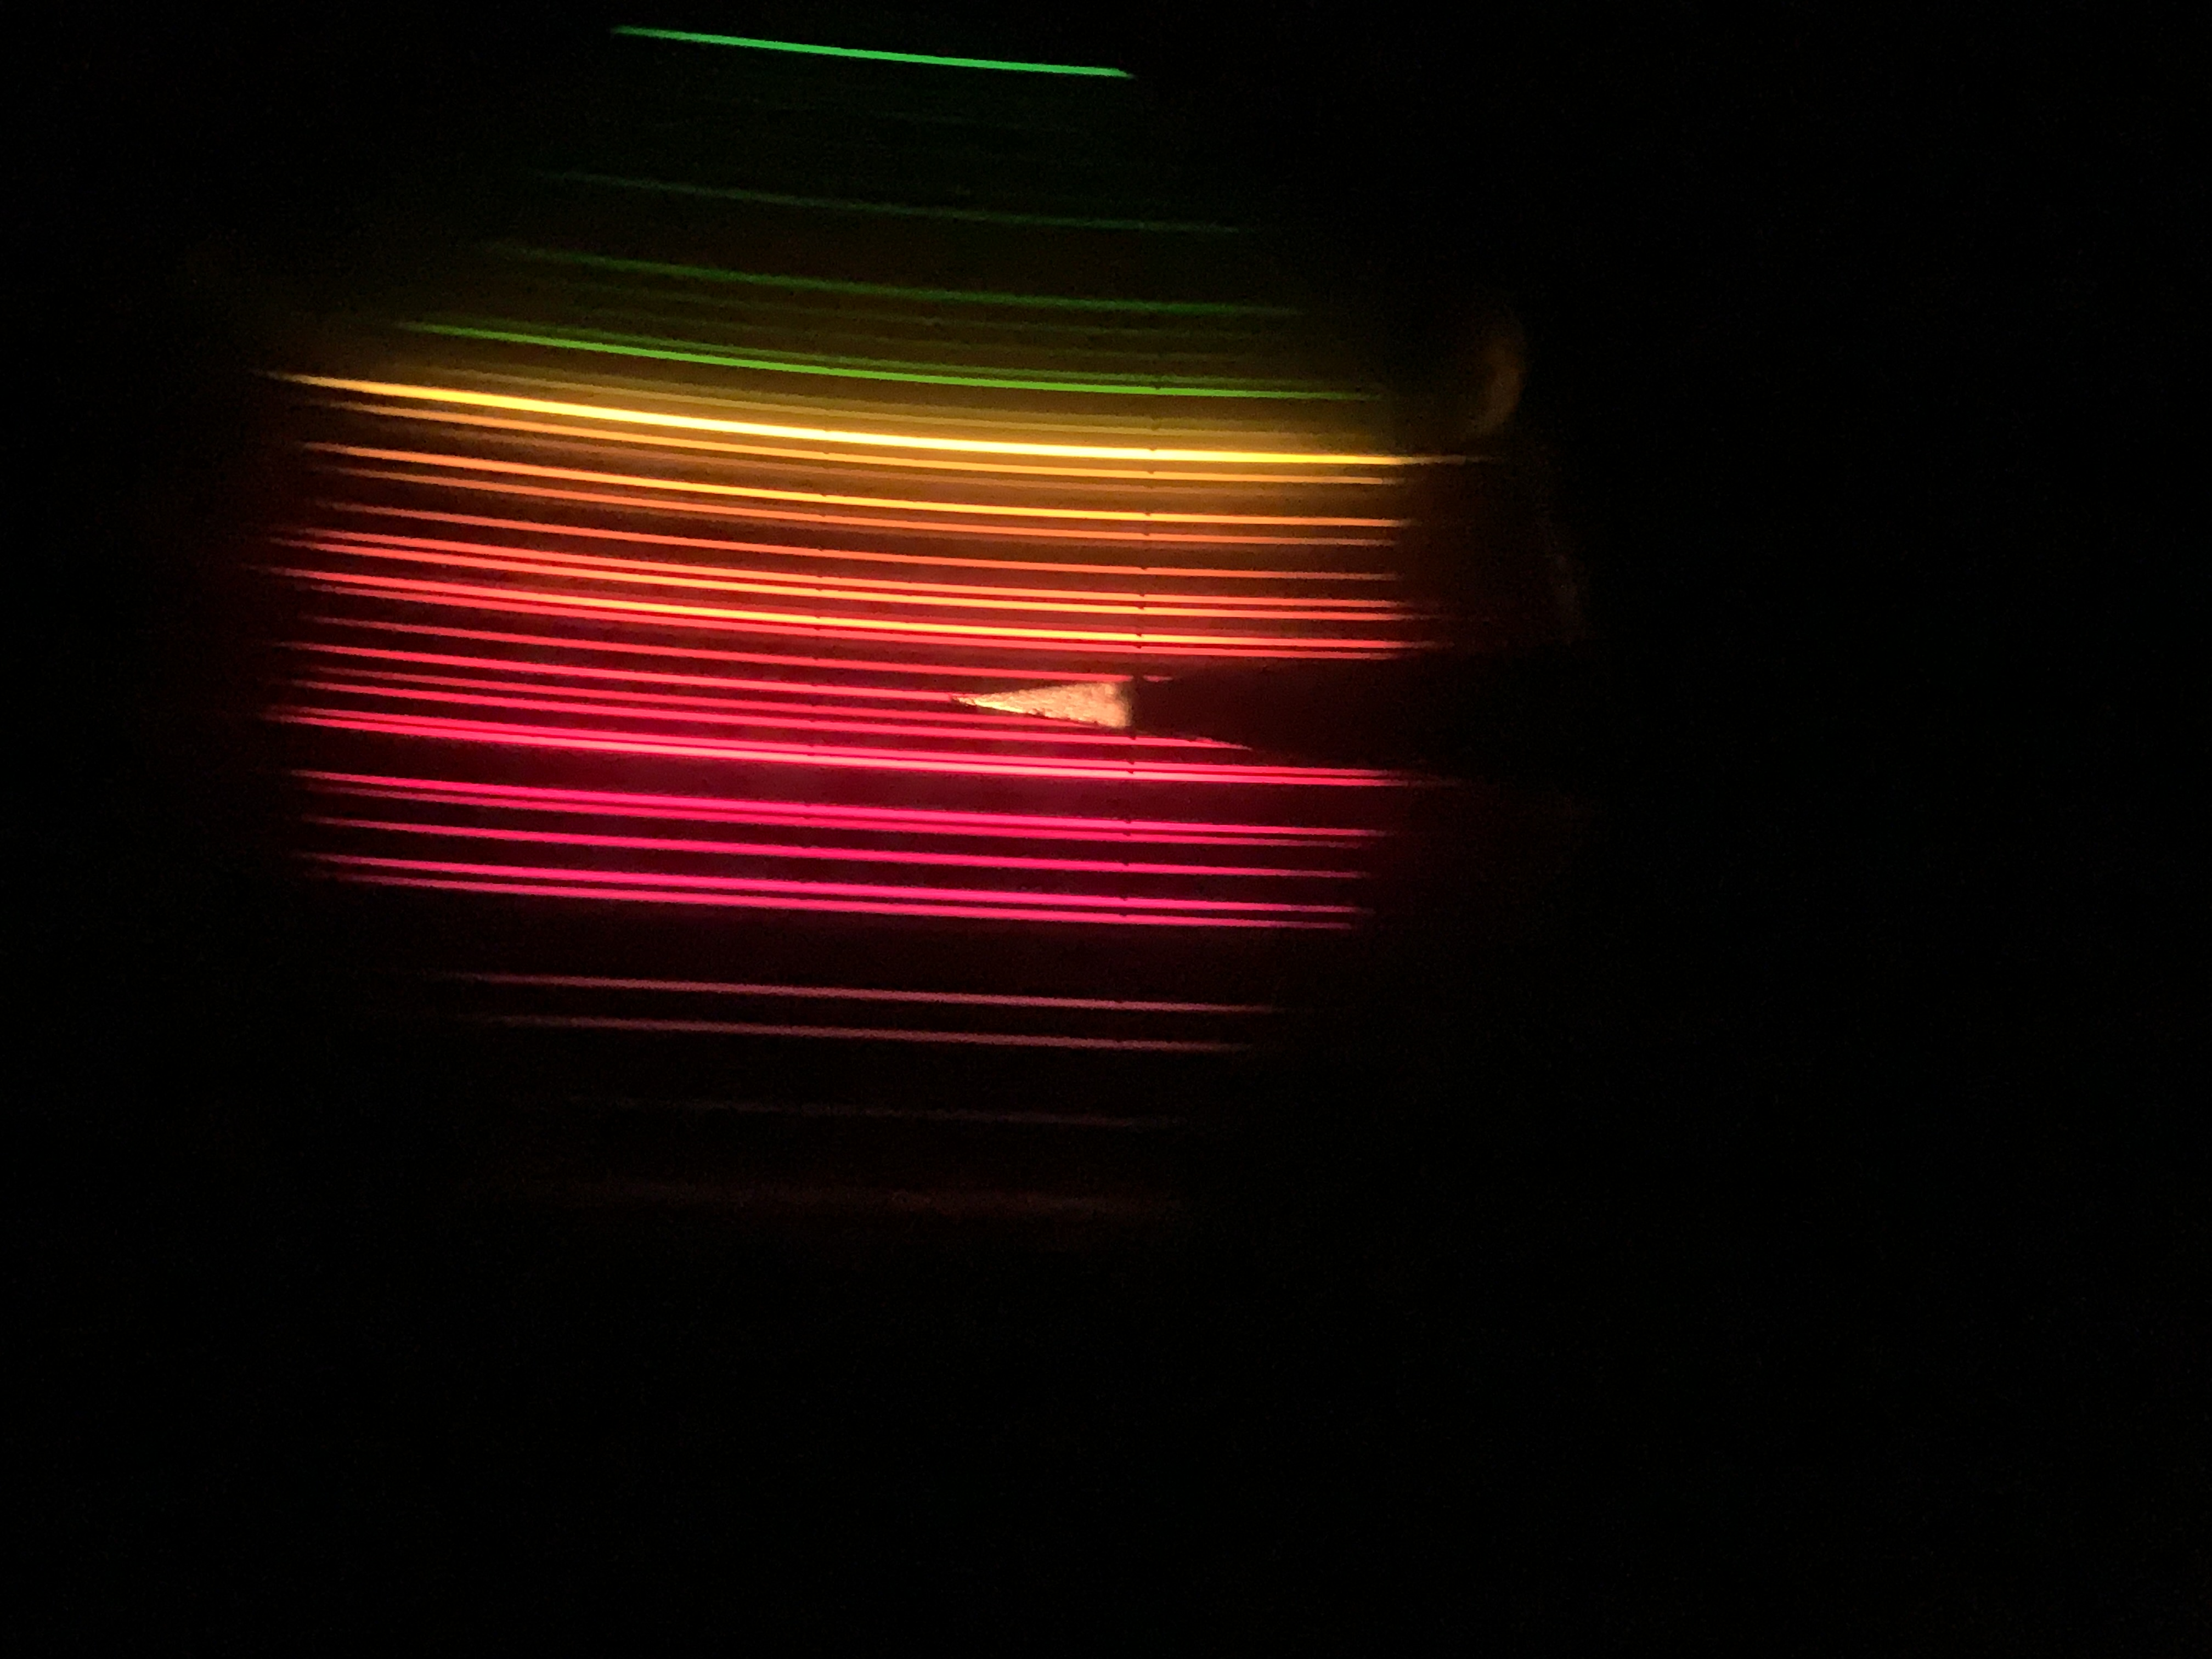
\includegraphics[angle=-90,  scale=0.075]{Спектр_неона.PNG}
		\caption{Спектр неона}
	\end{figure}
	
	\begin{figure}[h!]
		\centering
		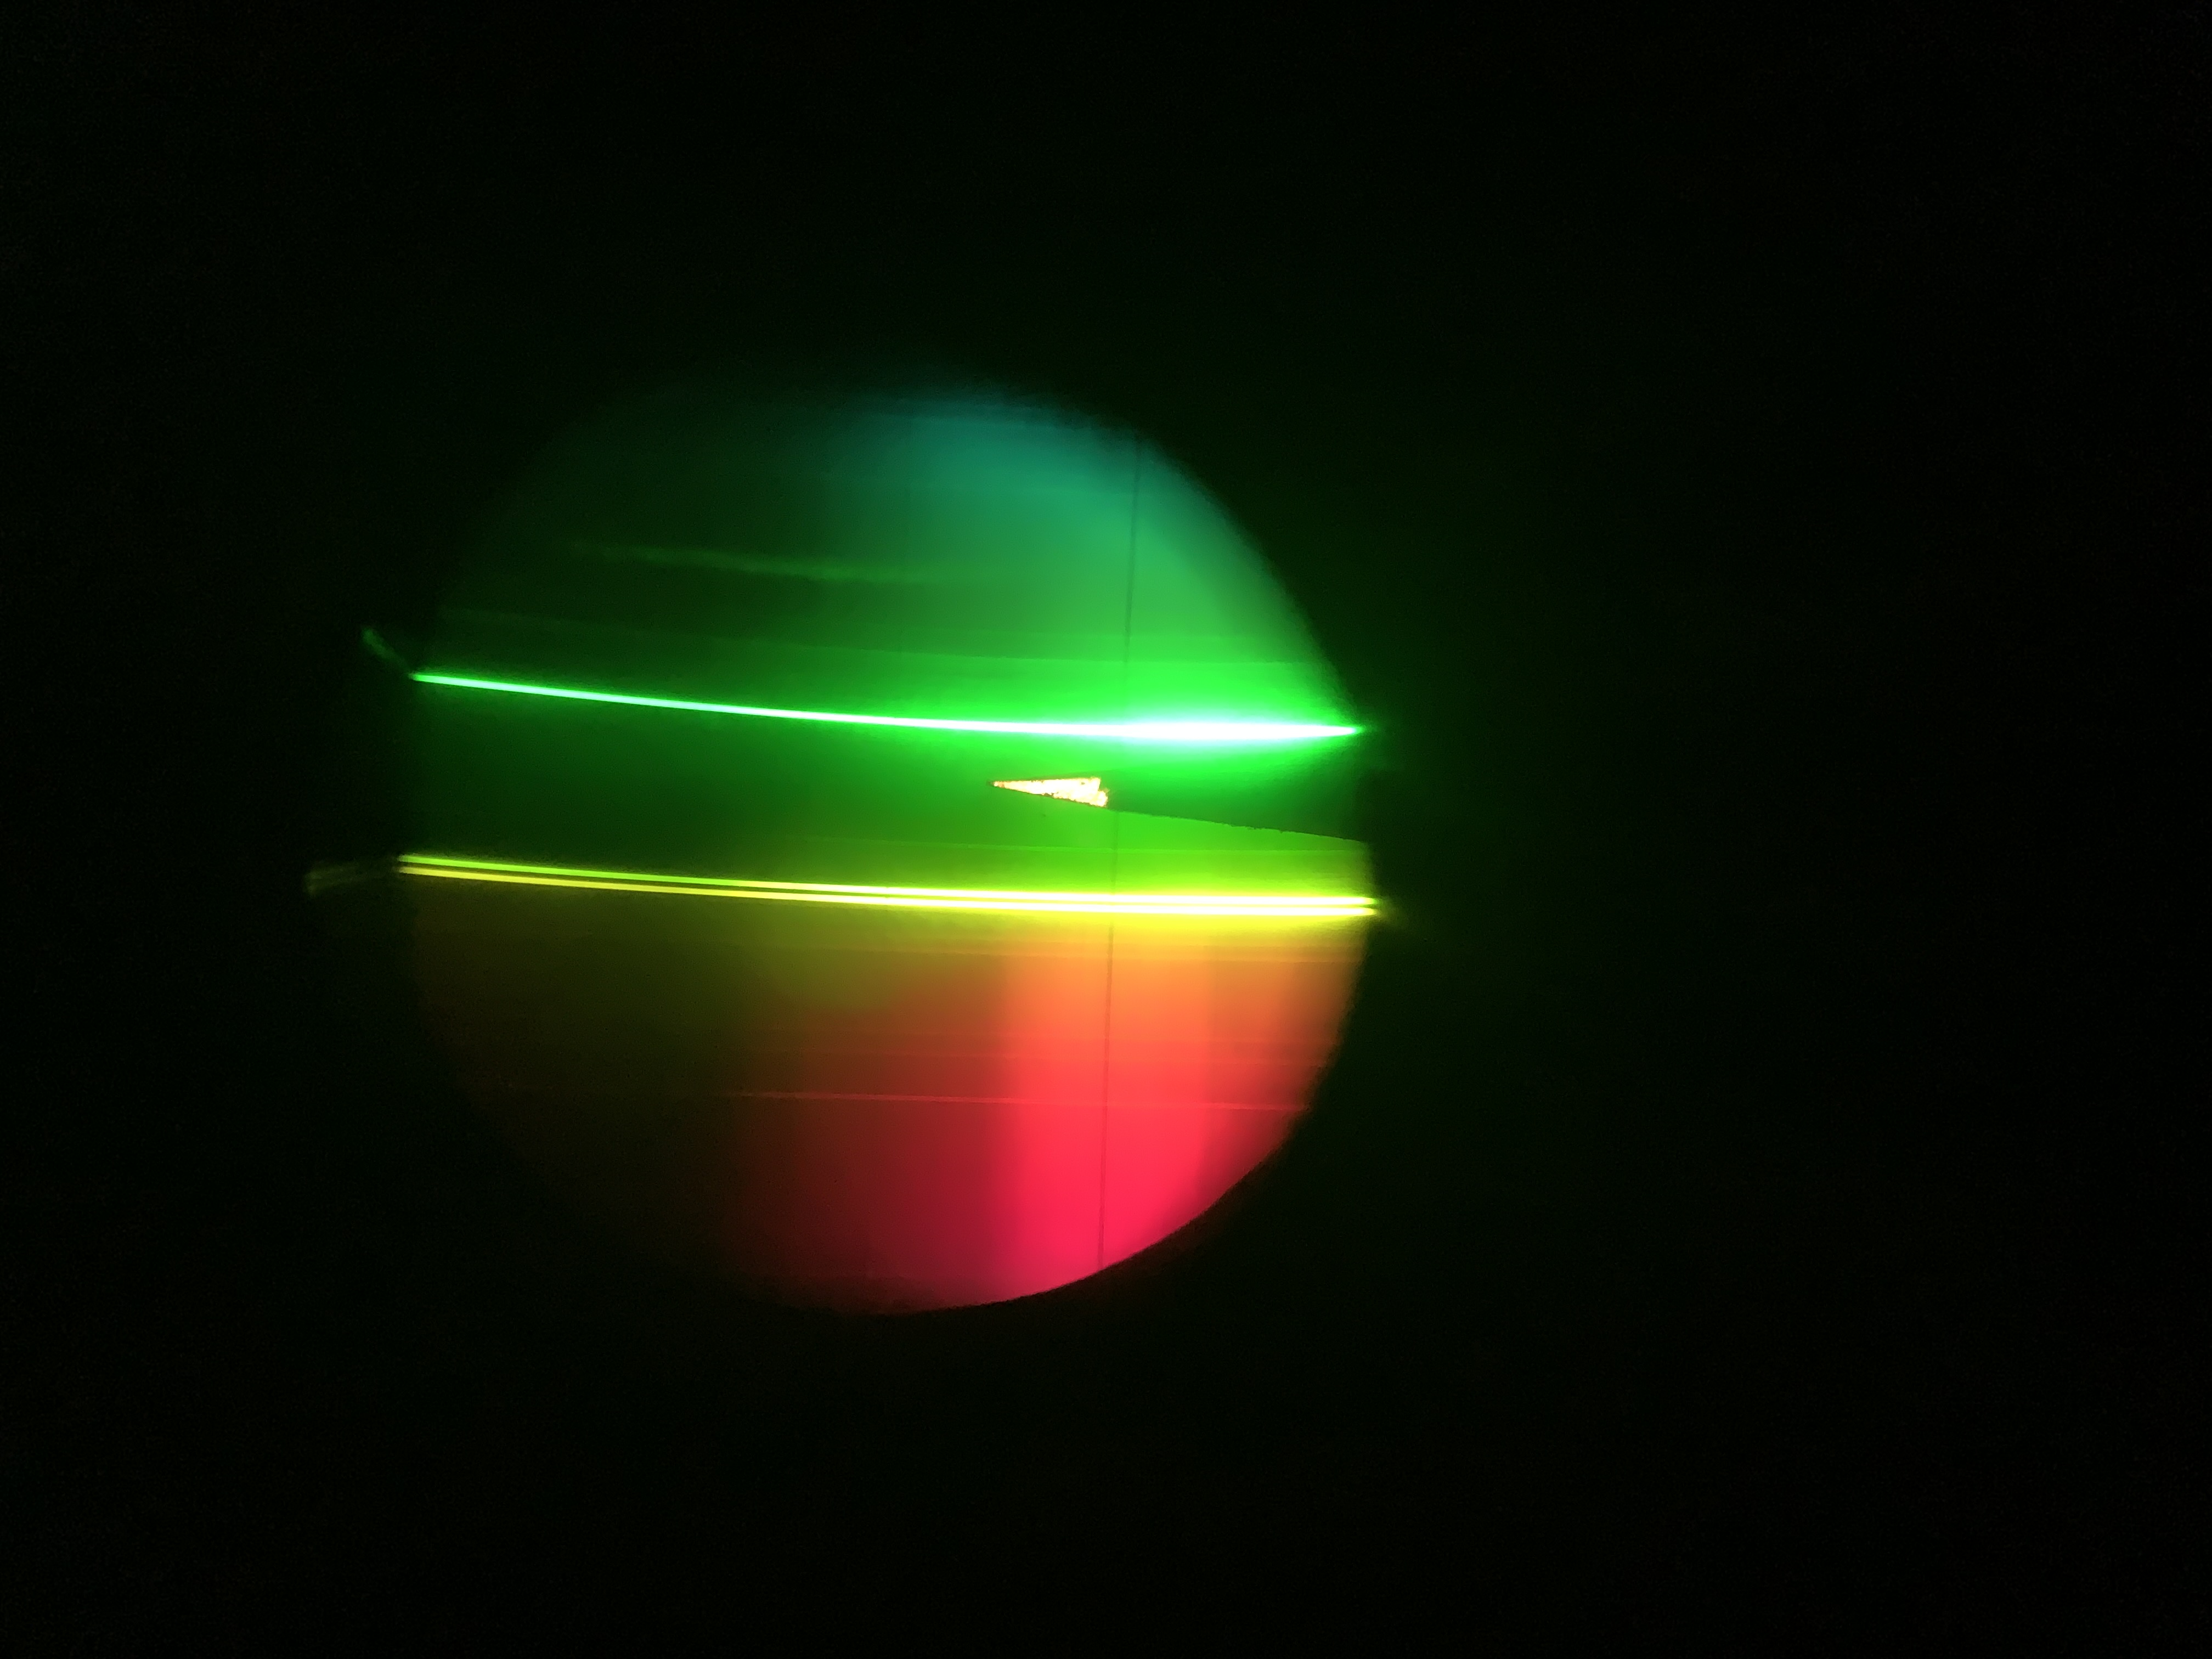
\includegraphics[angle=-90,  scale=0.075]{Спектр_йода.PNG}
		\caption{Спектр йода}
	\end{figure}

\newpage
	
	По таблице построим калибровочный график:

	\begin{figure}[h!]
		\centering
		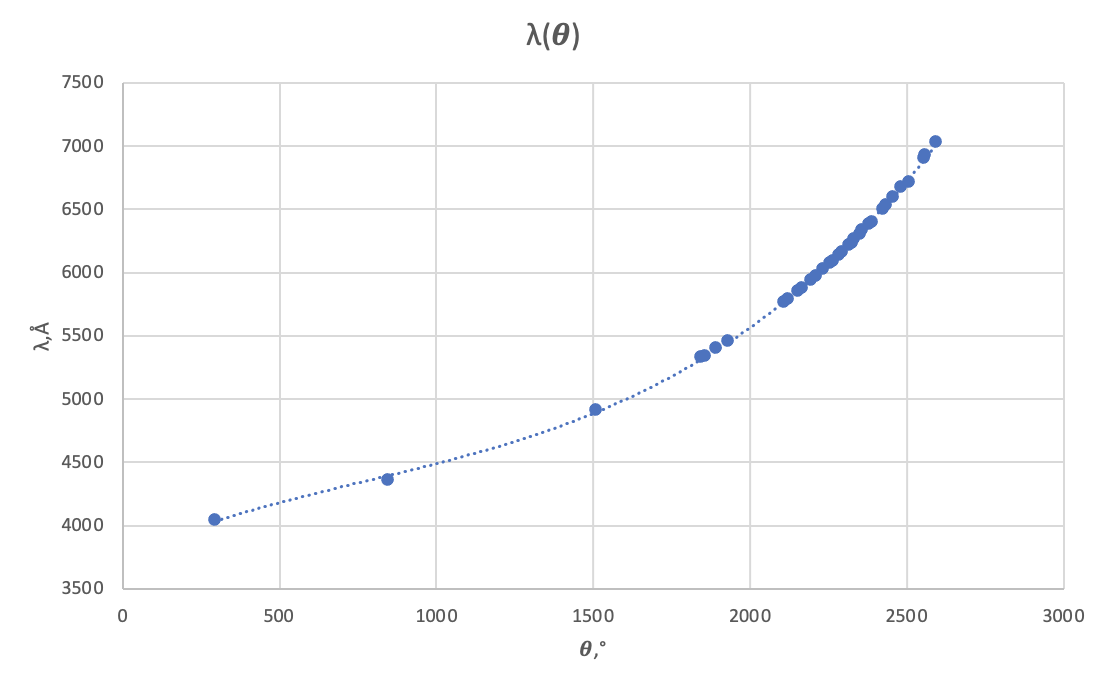
\includegraphics[scale=0.8]{График_1.PNG}
	\end{figure}

\item Измерим положение линий $H_{\alpha},  H_{\beta},  H_{\gamma},  H_{\delta}$,  затем с помощью калибровочного графика определим длины волн линий:

	\begin{figure}[h!]
		\centering
		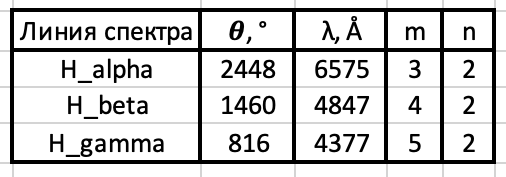
\includegraphics[scale=0.8]{Таблица_2.PNG}
	\end{figure}

Линию $H_{\delta}$ наблюдать не удалось из-за слабой интенсивности. 

Для проверки формулы сериальной закономерности построим график зависимости $1 / \lambda$ от $1/ n^2 - 1/m^2$:

	\begin{figure}[h!]
		\centering
		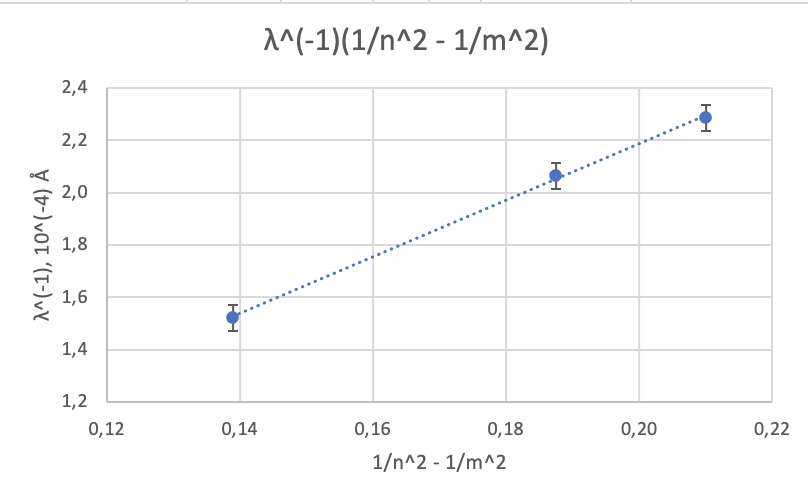
\includegraphics[scale=0.7]{График_2.PNG}
	\end{figure}
	
Для каждой из наблюдаемых линий водорода вычислим значение постоянной Ридберга, а затем определим ее среднее значение:

\[R_H^{(m)} = \left(\lambda_{m, n} Z^2 \left(\dfrac{1}{n^2} - \dfrac{1}{m^2}\right)\right)^{-1}\]

\[R_H^{\alpha} = (109502,3 \pm 163,1) \text{ см}^{-1}\]

\[R_H^{\beta} = (110034,2 \pm 215,2) \text{ см}^{-1}\]

\[R_H^{\gamma} = (108794,5 \pm 207,1) \text{ см}^{-1}\]

\[R_H = (109443,7 \pm 195,3) \text{ см}^{-1}\]

Теоретическая формула:

\[R_H^{\text{теор}} = \dfrac{m_e e^4}{4 \pi c \hbar^3} = 109726 \text{ см}^{-1}\]

\item Сопоставим наблюдаемый спектр йода со спектром поглощения.  Определим деления барабана монохроматора $\theta$,  соответствующие:

\begin{enumerate}

	\item линии $h \nu_{1, 0}$ -- одной из самых длинноволновых хорошо видимых линий поглощения:
    
		\[\theta_{1, 0} = (2230 \pm 2)^{\circ}\]
    
	\item линии $h \nu_{1, 5}$ -- шестой по счету от выбранной длинноволновой линии: 
	
		\[\theta_{1, 5} = (2132 \pm 2)^{\circ}\]
    
    \item линии $h \nu_{\text{гр}}$ -- началу сплошного спектра поглощения: 
    
		\[\theta_{1, 0} = (1770 \pm 2)^{\circ}\]
    
\end{enumerate}

	При помощи градуировочной кривой монохроматора определим длины волн линий поглощения йода и соответствующие энергии:
	
\[ \lambda_{1, 0} = (6495 \pm 9) \text{ \AA} \hspace{1cm} h \nu_{1, 0} = (1,921 \pm 0,03) \text{ эВ}\]

\[\lambda_{1, 5} = (6227 \pm 9) \text{ \AA} \hspace{1cm} h \nu_{1, 5} = (2,012 \pm 0,03) \text{ эВ}\]

\[\lambda_{\text{гр}} = (5443 \pm 9) \text{ \AA} \hspace{1cm} h \nu_{\text{гр}} = (2,301 \pm 0,03) \text{ эВ}\]

Вычислим энергию колебательного кванта возбужденного состояния молекулы йода:

\[h \nu_2 = \frac{h \nu_{1, 5} - h \nu_{1, 0}}{5}\]

\[h \nu_2 = (0,018 \pm 0,002) \text{ эВ}\]

Используя то,  что энергия колебательного кванта основного состояния $h \nu_1 = 0,027 \text{ эВ}$,  а энергия возбуждения атома $E_{\text{а}} = 0,94 \text{ эВ}$, вычислим:

\begin{enumerate}

    \item Энергию электронного перехода $h \nu_{\text{эл}}$:
	    
		\[h \nu_{n_1, n_2} = h\nu_{\text{эл}} + h \nu_2 \left( n_2 + \dfrac{1}{2} \right) - h \nu_1 \left( n_1 + \dfrac{1}{2} \right)\]
    
		\[h \nu_{\text{эл}} = h \nu_{1, 0} + \dfrac{3}{2} h \nu_1 - \dfrac{1}{2} h \nu_2 \]
    
		\[h \nu_{\text{эл}} = (1,952 \pm 0,005) \text{ эВ}\]
		
    \item Энергию диссоциации молекулы в основном состоянии $D_1$:
    
    \[D_1 = h \nu_{\text{гр}} - E_{\text{а}}\]
    
    \[D_1 = (1,361 \pm 0,006) \text{ эВ}\]
    
    \item Энергию диссоциации молекулы в возбужденном состоянии $D_2$:
    
    \[D_2 = h \nu_{\text{гр}} - h \nu_{\text{эл}}\]
    
    \[D_2 = (0,349 \pm 0,009) \text{ эВ}\]
    
\end{enumerate}

\end{enumerate}

\textbf{Вывод:}\\\par

В результате выполнения лабораторной работы:

\begin{enumerate}
	
	\item Проверена справедливость формулы сериальной закономерности.
	
	\item При исследовании спектра водорода наблюдались линии,  соответствующие серии Бальмера.  Последнюю линию $H_{\delta}$ не удалось увидеть в силу ее слабой интенсивности,  однако значения оставшихся достаточно точно совпадают с табличными:
	
		\[\lambda_{\alpha} =  (657,5 \pm 1,5) \text{ нм} \hspace{1cm} \lambda_{\alpha}^{\text{теор}} = 656,3 \text{ нм}\]
		
		\[\lambda_{\beta}=  (484,7 \pm 1,5) \text{ нм} \hspace{1cm} \lambda_{\beta}^{\text{теор}} = 486,1 \text{ нм}\]
			
		\[\lambda_{\gamma} =  (437,7 \pm 1,5) \text{ нм} \hspace{1cm} \lambda_{\gamma}^{\text{теор}} = 434,1 \text{ нм}\]	
					
	\item Вычислена постоянная Ридберга,  которая достаточно точно совпадает с табличным:
	
		\[R_H = (109443,7 \pm 195,3) \text{ см}^{-1} \hspace{1cm} R_H^{\text{теор}} = 109726 \text{ см}^{-1}\]
	
	\item Для молекулы йода были вычислены:
	
		\begin{enumerate}
		
			\item Энергия электронного перехода:
			
				\[h \nu_{\text{эл}} = (1,952 \pm 0,005) \text{ эВ}\]
			
			\item Энергия диссоциации молекулы в основном состоянии:
			
				 \[D_1 = (1,361 \pm 0,006) \text{ эВ}\]
			
			\item Энергию диссоциации молекулы в возбужденном состоянии:	
			
				\[D_2 = (0,349 \pm 0,009) \text{ эВ}\]
		
		\end{enumerate}
		    
\end{enumerate}

\end{document}